\subsection{Directions, gains, and finite-window occupancy}
We distinguish the direction used for measurement from the statistic applied to its gain law. For plain SGD let $H_B(\theta)=\nabla^2 L_B(\theta)$. A unit direction $q$ defines the scalar compression
\begin{equation}
 a_B(q;\theta)=q^\top(I-\eta H_B(\theta))q=1-\eta q^\top H_B(\theta)q.
\end{equation}
The batch-gradient measurement uses $q_B=g_B/\|g_B\|$, where $g_B=\nabla L_B(\theta)$; its sampled curvature is $s_B=g_B^\top H_Bg_B/(g_B^\top g_B)$. This is the batch-gradient curvature statistic used by the vision heatmaps. The gain law is formed before taking moments: $\mathbb E|1-\eta s_B|^p$ is not $|1-\eta\mathbb E s_B|^p$. An unweighted average of these Rayleigh quotients also differs in general from a gradient-norm-weighted batch-sharpness ratio.

For the occupancy measurement, $q_*$ is a checkpoint-fixed leading full-data Hessian Ritz vector and $\theta_*$ is the checkpoint parameter vector, not an estimated minimizer. Every histogram uses $z_t=q_*^\top(\theta_t-\theta_*)$. We separately recompute a leading Ritz vector $q_1(t)$ and report $|q_1(t)^\top q_*|$. The plotting frame remains fixed even when the evolving eigenvector changes. Fixed checkpoint-gradient and random directions provide additional scalar comparisons.

For any one declared gain pool, we report four generalized means:
\begin{equation}
 \mathsf H=\bigl\langle |a|^{-1}\bigr\rangle^{-1},\qquad
 \mathsf G=\exp\langle\log|a|\rangle,\qquad
 \mathsf A_1=\langle|a|\rangle,\qquad
 \mathsf A_2=\sqrt{\langle|a|^2\rangle}.
\end{equation}
Their reference is one; $\Lambda=\log\mathsf G$ has reference zero. On the same pool $\mathsf H\leq\mathsf G\leq\mathsf A_1\leq\mathsf A_2$. Here $\mathsf H$ is the reciprocal of the inverse moment, so harmonic expansion means $\mathsf H>1$, equivalently $\langle|a|^{-1}\rangle<1$. This convention must not be confused with denoting the inverse moment itself by $H$. Inverse gains are not clipped; finite samples do not certify existence of a population negative moment.

A scalar compression is also distinct from a norm gain $\|(I-\eta H_B)q\|$. To assess transported perturbations we propagate $v_{t+1}=(I-\eta H_{B_t}(\theta_t))v_t$, normalizing only its length between updates. The plotted cumulative sum is $\sum_{t<T}\log(\|v_{t+1}\|/\|v_t\|)$ before normalization. This preserves directional coupling; resetting $v_t$ to $q_*$ would measure a different object.

\paragraph{Current observation.}
The CIFAR-10 SiLU MLP continuation uses IID subsets of size 4096, learning rate 0.04, and 4096 additional updates from checkpoint 10001. Loss on its 8192-example training subset decreases from 0.02485 to 0.00935. Fixed-coordinate windows show alternating two-lobe occupancy while the late transported log-growth rate is approximately $+0.00642$ per update. The late fixed-axis scalar log average can nevertheless be negative. New eigenvector probes show variable alignment, including sharp decreases; they do not support a permanently fixed leading eigendirection. The paired probes also show phase-dependent harmonic gains. These observations establish finite-window coexistence, not an invariant neural distribution or a universal harmonic-to-bimodal transition. The previously selected CNN fixed-axis candidate fails confirmation under the same shape screen.

\paragraph{Across architectures and optimizers.}
The architecture-level figures combine runs without separate seed panels. Heatmap cells average per-run statistics from the last three available checkpoints; different cells can use different occupied states and times. The gain-law comparison explicitly labels its architecture-specific learning rates. For GPT 168M on the FineWeb-Edu subset, distinguish raw Hessian/GGN probes from frozen-Adam probes. With $D=\operatorname{diag}(1/(\sqrt{\hat v}+\epsilon))$ fixed, the latter use
\begin{equation}
 s_{D,B}=\frac{(Dg_B)^\top H_B(Dg_B)}{g_B^\top Dg_B},\qquad a_{D,B}=1-\eta s_{D,B},
\end{equation}
with $H_B$ replaced by GGN when specified. This is a scalar compression in symmetrically preconditioned coordinates; it is not the full Adam state-space Jacobian. All GPT parents process 16.384 million tokens.


\begin{figure}[p]\centering
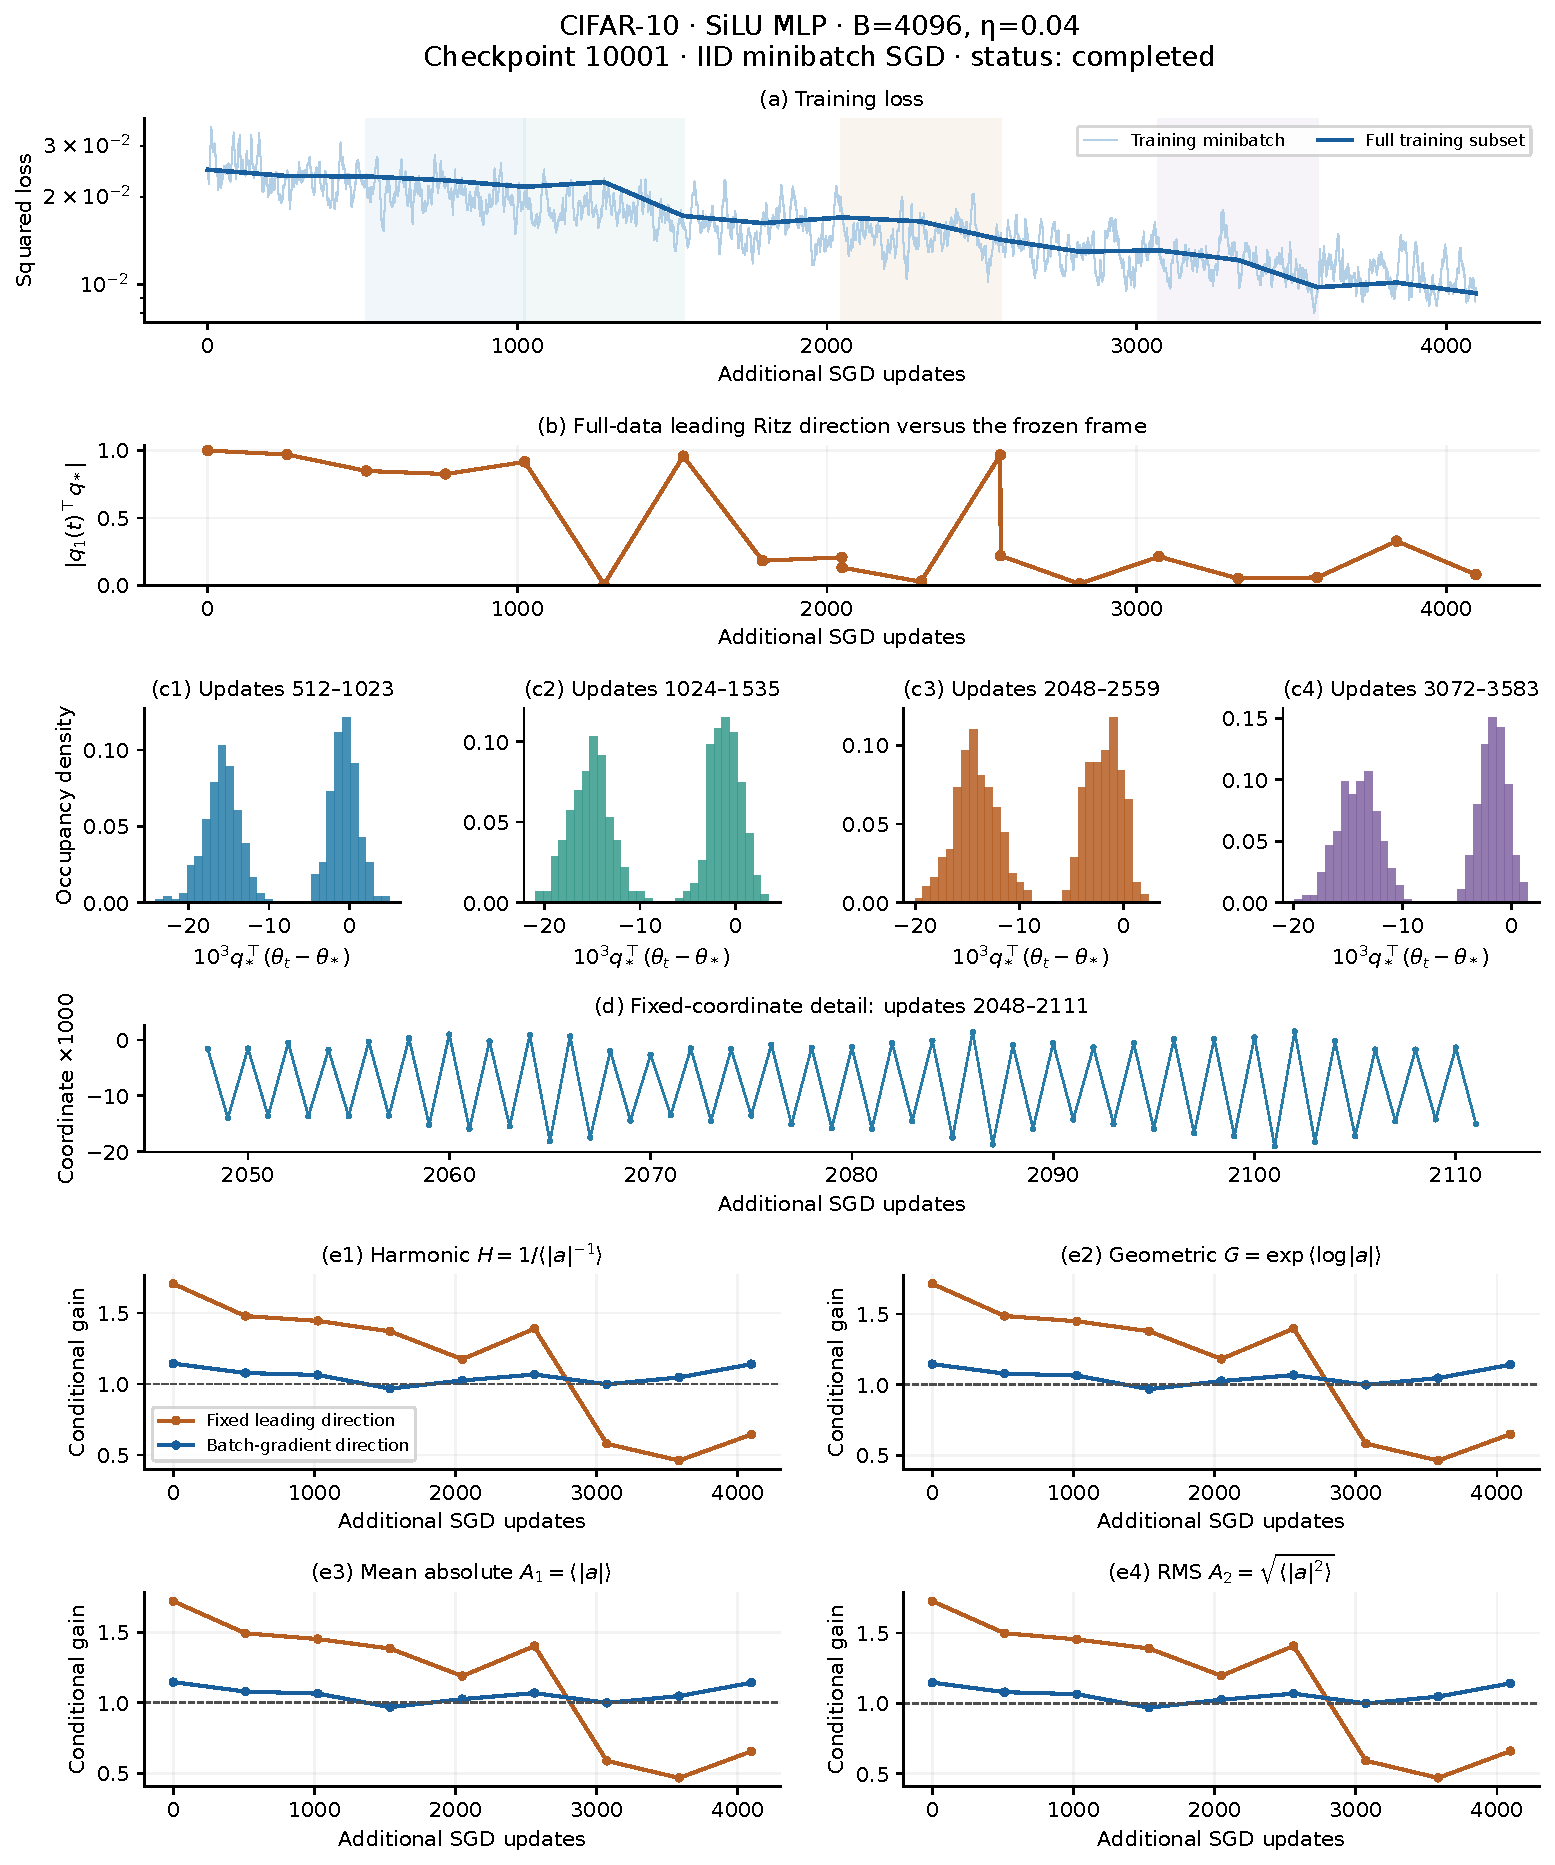
\includegraphics[width=\linewidth,height=0.78\textheight,keepaspectratio]{img/current_results/fig01_mlp_loss_alignment_bimodality.pdf}
\caption{The center and plotting direction are fixed at the parent checkpoint. All runs use IID subsets, original parent learning rate, and the full 8192-example training subset. Curvature matrices in the alignment panel use that same subset. Histograms use four declared 512-update intervals and 30 bins without selecting intervals by modality. The short trace uses updates2048--2111. Gain ladders use fresh minibatches at each plotted state: fixed-axis compression versus batch-gradient compression, each summarized by H,G,A1,A2. No propagated-tangent panel and no static ladder panels are included. Sparse even-update conditional probes do not average over oscillation phases; they do not establish stationarity or a full-network Lyapunov exponent. Alignment is measured, not assumed, and Ritz extremality is not certified. The original anchor uses128 fresh draws at zero and24 at subsequent even states512k.}
\label{fig:current-fig01-mlp-loss-alignment-bimodality}
\end{figure}\clearpage

\begin{figure}[p]\centering
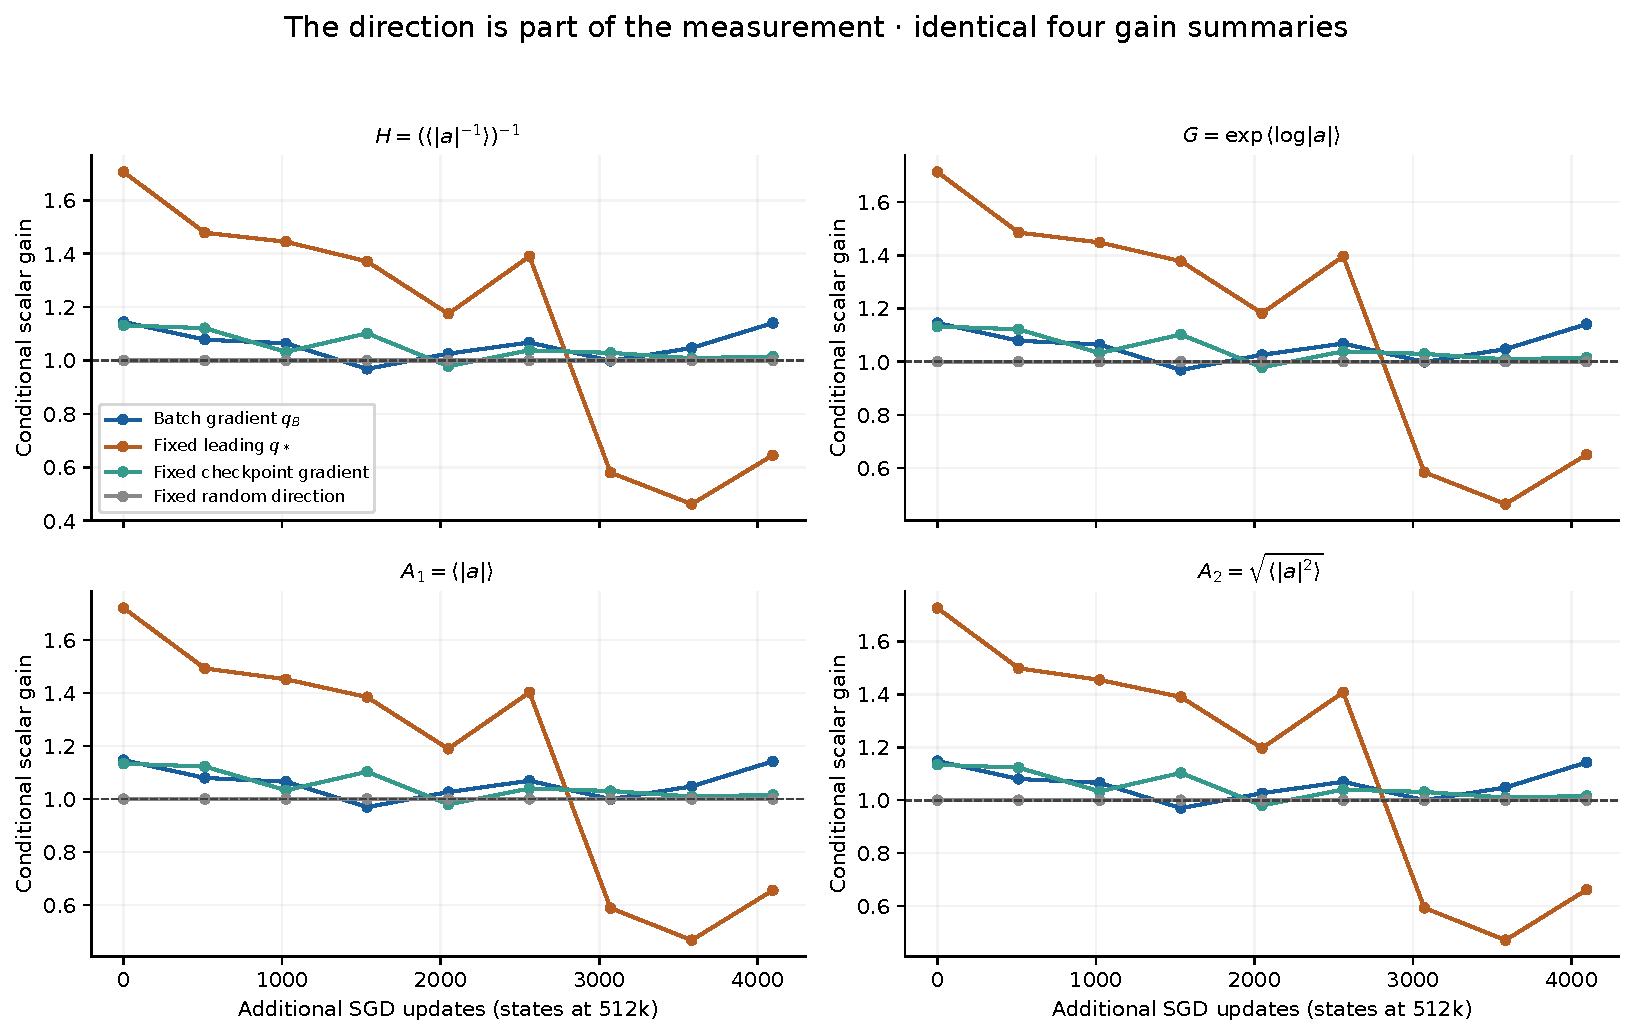
\includegraphics[width=\linewidth,height=0.78\textheight,keepaspectratio]{img/current_results/fig02_direction_resolved_ladder.pdf}
\caption{Fresh conditional minibatch probes at each displayed fixed state, using the same draws across directions. There are 128 draws at update zero and 24 at other displayed states. Only states at multiples of 512 are displayed here; the adjacent phase appears in Figure 3. The batch-gradient direction changes with the sampled batch. All other directions are checkpoint-fixed. Geometric gain G=exp(Lambda) shares the unit reference with H, A1 and A2. Finite H does not establish a finite population inverse moment.}
\label{fig:current-fig02-direction-resolved-ladder}
\end{figure}\clearpage

\begin{figure}[p]\centering
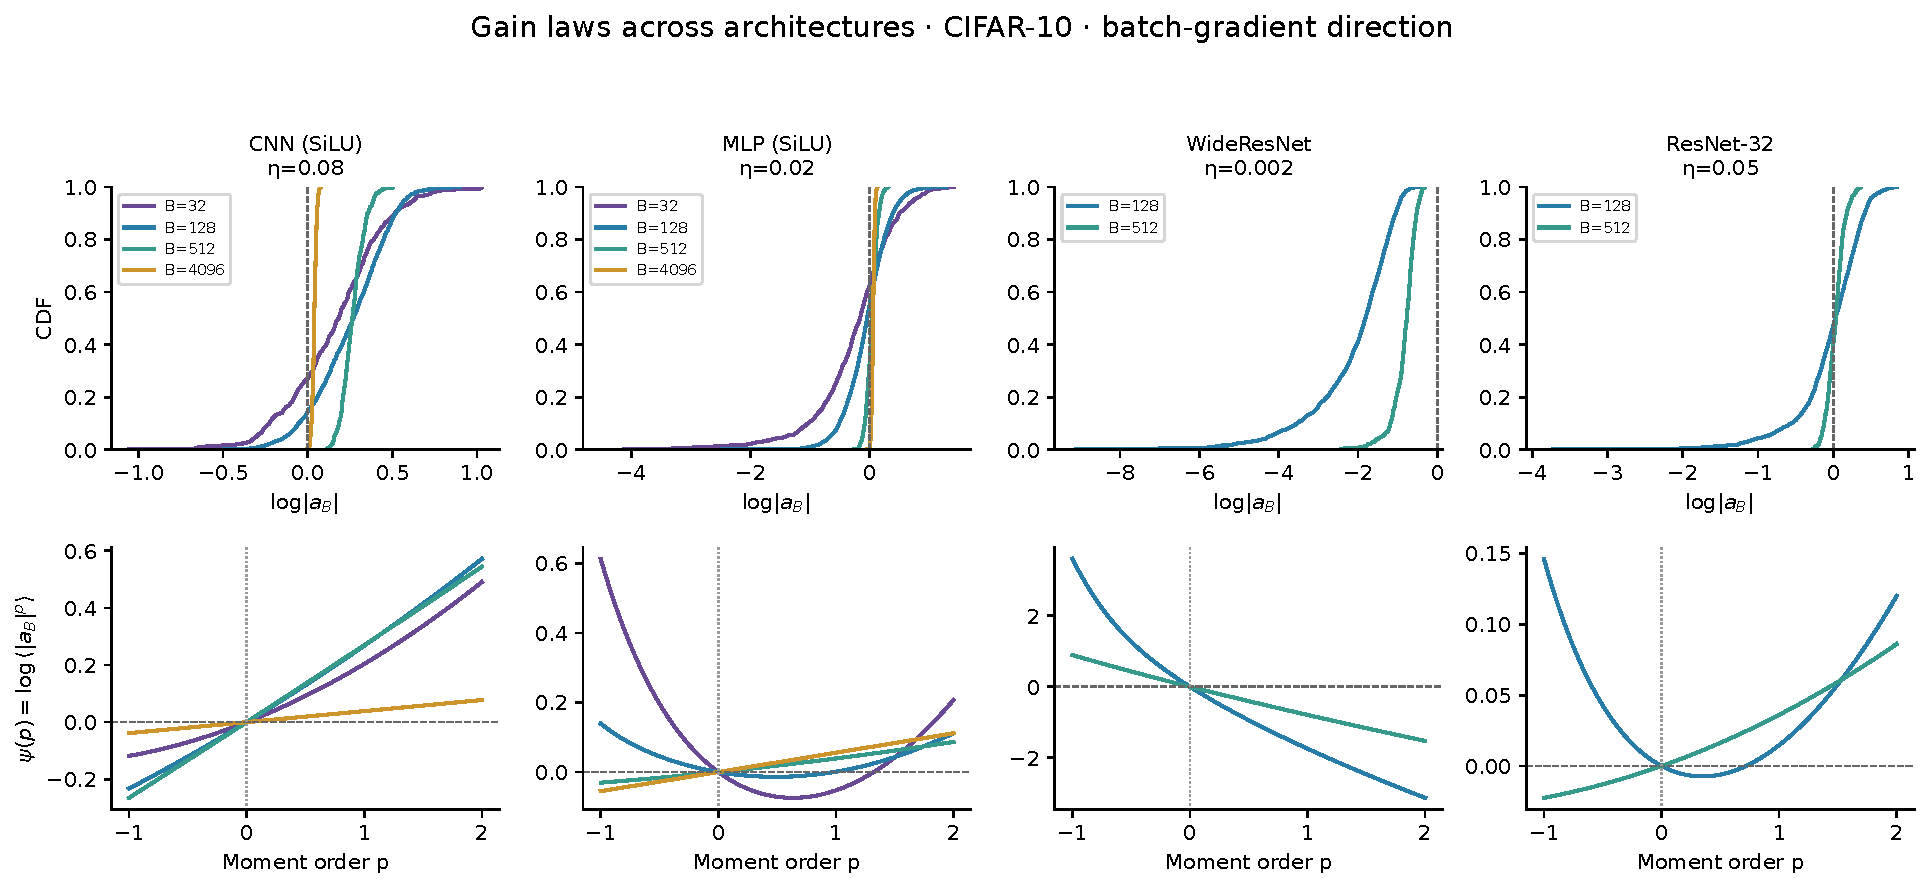
\includegraphics[width=\linewidth,height=0.78\textheight,keepaspectratio]{img/current_results/fig04_cross_architecture_gain_laws.pdf}
\caption{Batch-gradient scalar gains at update 20000 and matched training/probe batch size. Curves average within-run CDFs or log moments equally across available runs; this is not the log moment of pooled gains. No separate seed panels. Architecture-specific step sizes are labeled; this is not a controlled comparison changing architecture alone. Only measured final-checkpoint cases are shown; the full grids retain earlier/pre-escape observations. Positive and negative moments summarize gain distributions, not parameter-coordinate histograms.}
\label{fig:current-fig04-cross-architecture-gain-laws}
\end{figure}\clearpage

\begin{figure}[p]\centering
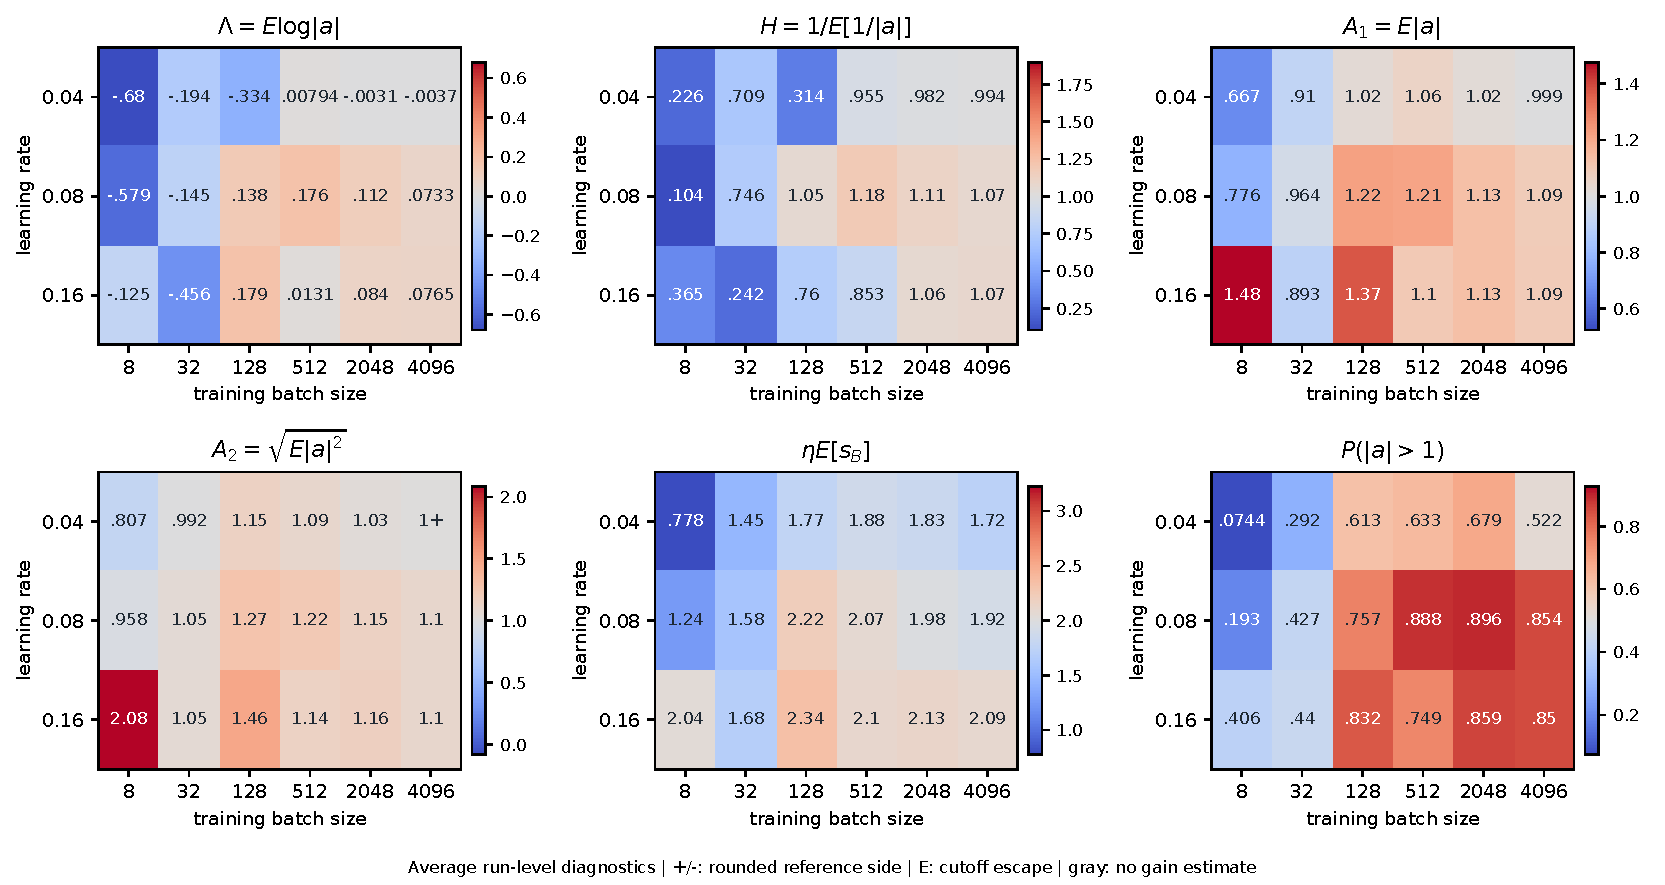
\includegraphics[width=\linewidth,height=0.78\textheight,keepaspectratio]{img/current_results/cnn_silu_grid_eta_batch.pdf}
\caption{\textbf{CNN with SiLU | stability grid over batch size and step size.} Axes are actual training learning rate and batch size. The six panels show Lambda, H, A1, A2, eta E[s\_B], and the fraction of expanding gains. Each cell averages run-level statistics from the final three available checkpoints; time windows can differ across settings and runs. Color centers are 0, 1, 1, 1, 2, and 0.5. Curvature and expansion-fraction centers are references, not full-network stability tests. A trailing +/- preserves the side of a reference after rounding. Gray means no gain estimate; E marks a recorded escape, including pre-escape estimates. Finite H does not establish population inverse-moment finiteness.}
\label{fig:current-cnn-silu-grid-eta-batch}
\end{figure}\clearpage

\begin{figure}[p]\centering
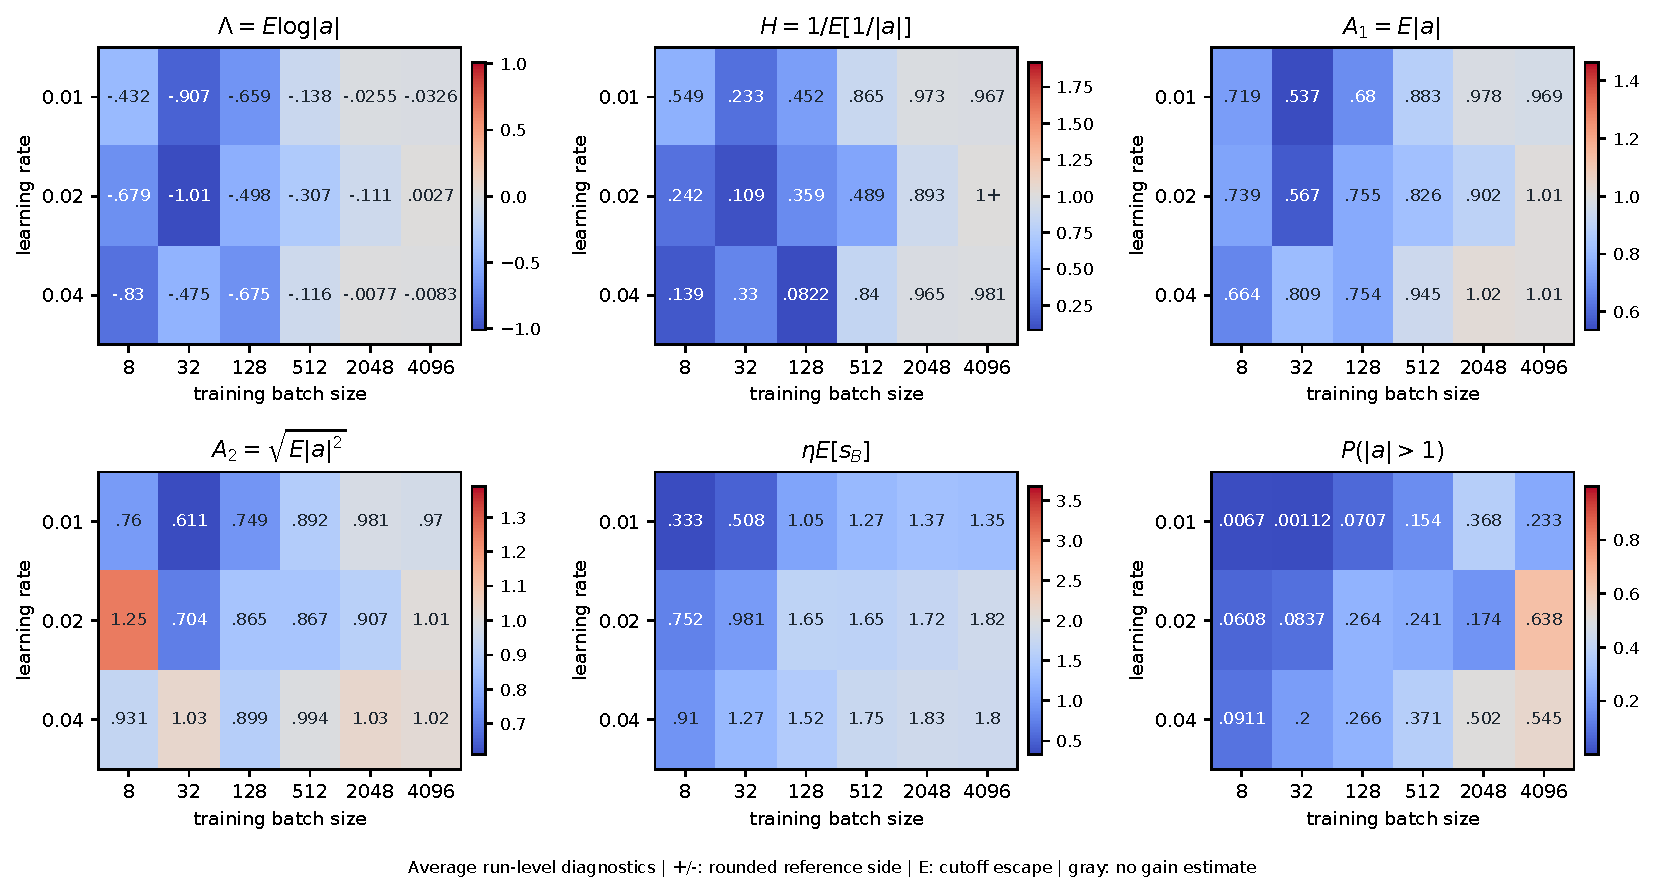
\includegraphics[width=\linewidth,height=0.78\textheight,keepaspectratio]{img/current_results/mlp_silu_grid_eta_batch.pdf}
\caption{\textbf{MLP, 2 x 512 (SiLU) | stability grid over batch size and step size.} Axes are actual training learning rate and batch size. The six panels show Lambda, H, A1, A2, eta E[s\_B], and the fraction of expanding gains. Each cell averages run-level statistics from the final three available checkpoints; time windows can differ across settings and runs. Color centers are 0, 1, 1, 1, 2, and 0.5. Curvature and expansion-fraction centers are references, not full-network stability tests. A trailing +/- preserves the side of a reference after rounding. Gray means no gain estimate; E marks a recorded escape, including pre-escape estimates. Finite H does not establish population inverse-moment finiteness.}
\label{fig:current-mlp-silu-grid-eta-batch}
\end{figure}\clearpage

\begin{figure}[p]\centering
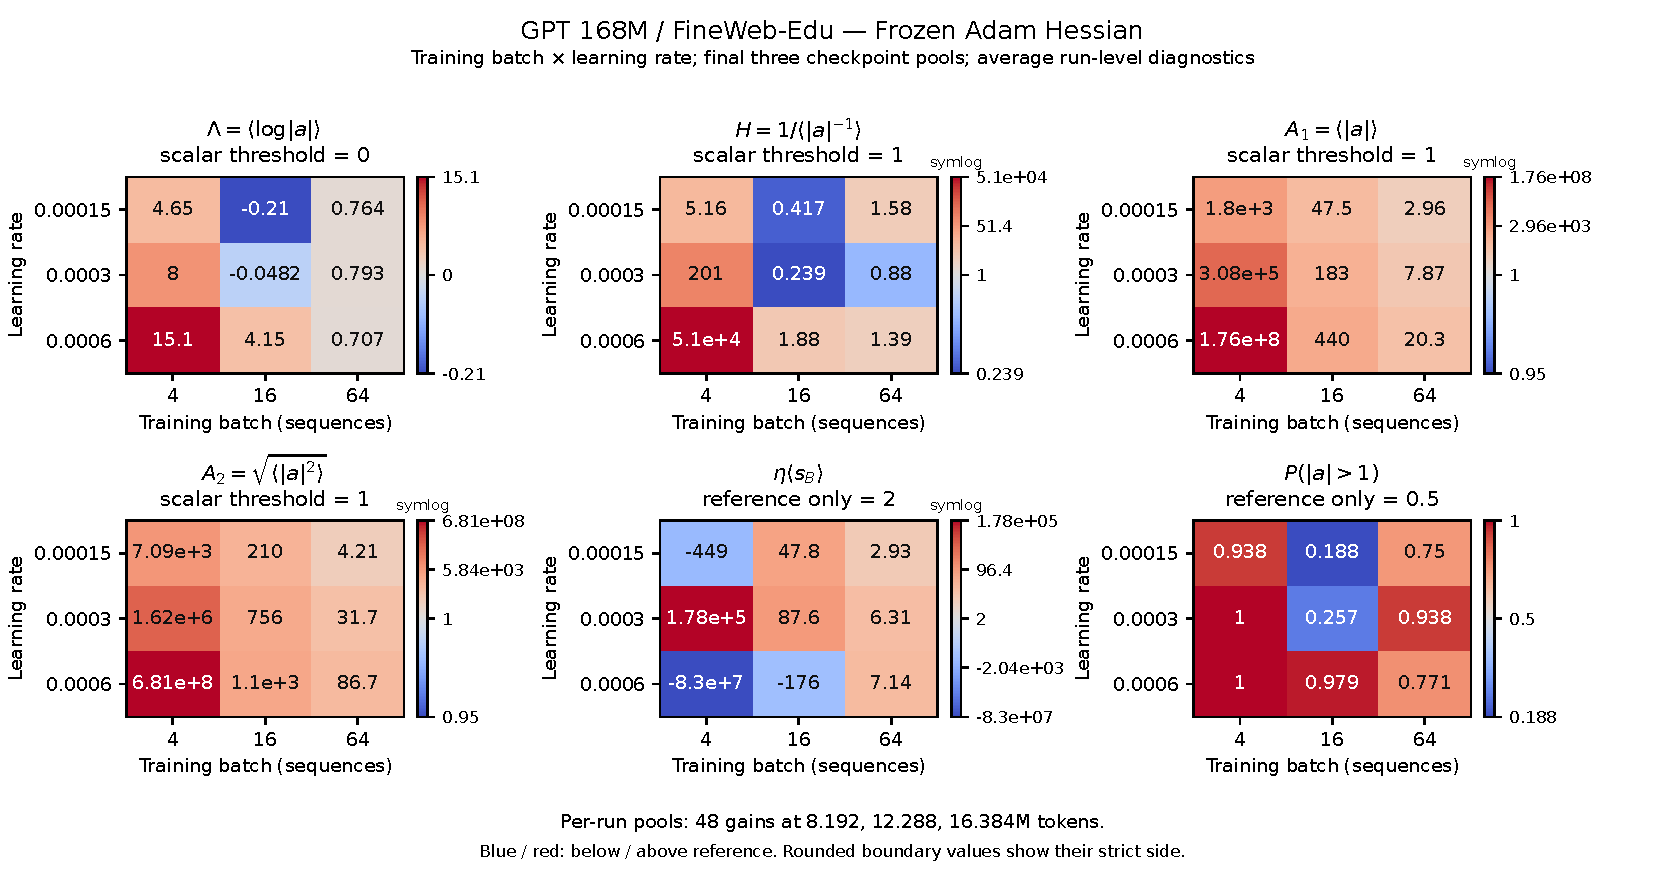
\includegraphics[width=\linewidth,height=0.78\textheight,keepaspectratio]{img/current_results/gpt_grid03_frozen_adam_hessian.pdf}
\caption{\textbf{GPT / FineWeb-Edu: batch--step-size grid, frozen adam hessian.} Frozen Adam Hessian; all nine batch-rate cells retained. Values average run-level statistics from final-three-checkpoint pools at 8.192, 12.288 and 16.384 million tokens. Blue/red means below/above the panel reference. Pools contain 48 Hessian or 24 GGN gains per run. Annotations use three significant figures, with strict inequalities when rounded to a threshold. Symlog colorbars retain extreme values; ticks use original units. Eta E[s\_B]=2 and P(|a|>1)=0.5 are references, not stability certificates. Small inverse-moment samples do not establish population finiteness or stationarity. Parents use Adam: raw metrics are scalar SGD counterfactuals; frozen metrics exclude momentum and preconditioner evolution. Neither is a full-Adam Jacobian.}
\label{fig:current-gpt-grid03-frozen-adam-hessian}
\end{figure}\clearpage
